\section{Problem 2}

\subsection{Question}
\vspace*{10pt}
We know the group split in two different groups.  Suppose the
disagreements in the group were more nuanced -- what would the clubs
look like if they split into groups of 3, 4, and 5?

\subsection{Answer}
The Edge Betweenness algorithm was run for target clusterings of three, four and five and the results are in Figures \ref{fig:cluster3}, \ref{fig:cluster4}, and \ref{fig:cluster5}.

\begin{figure}[h!]
\centering
\fbox{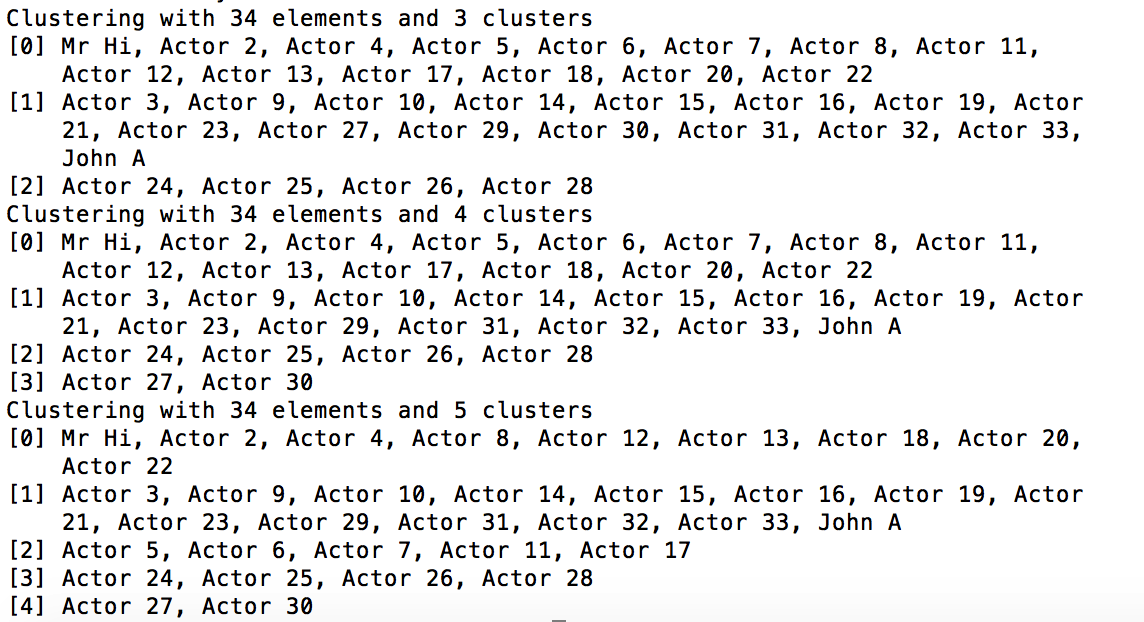
\includegraphics[scale=0.375]{q2/fig3.png}}
\caption{Groups Predicted by Girvan \& Newman Betweenness Clustering from Listing \ref{listing:karate}}
\label{fig:output3}
\end{figure}

\begin{figure}[h!]
\centering
\fbox{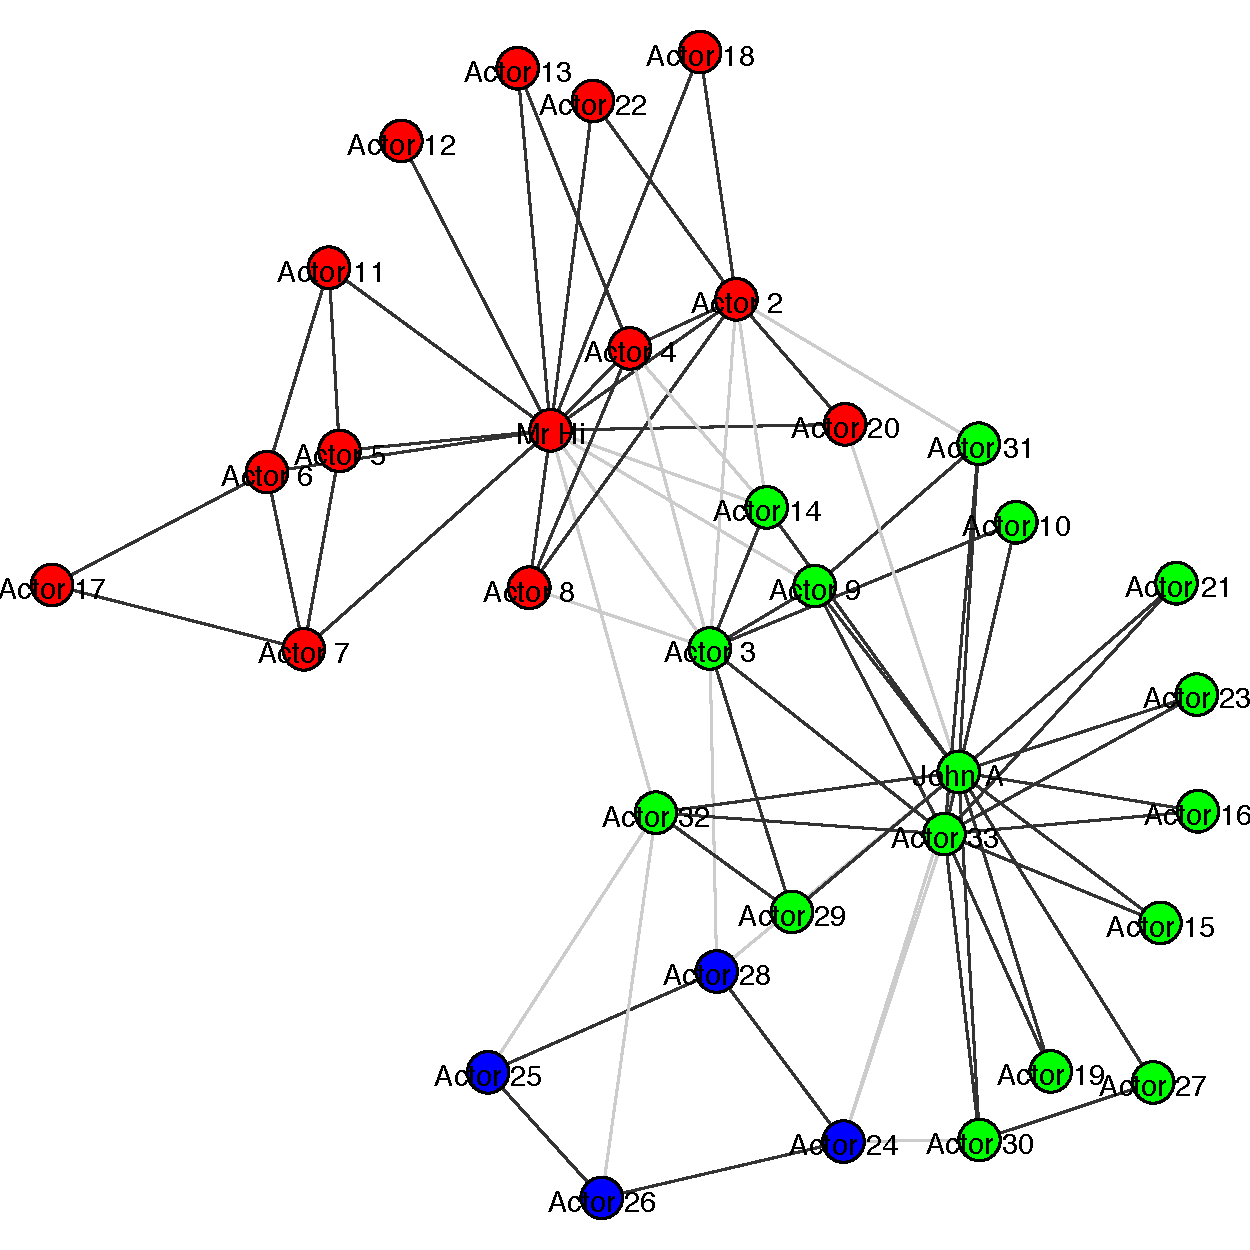
\includegraphics[scale=0.65]{q2/cluster3.pdf}}
\caption{3-Cluster Prediction}
\label{fig:cluster3}
\end{figure}

\begin{figure}[h!]
\centering
\fbox{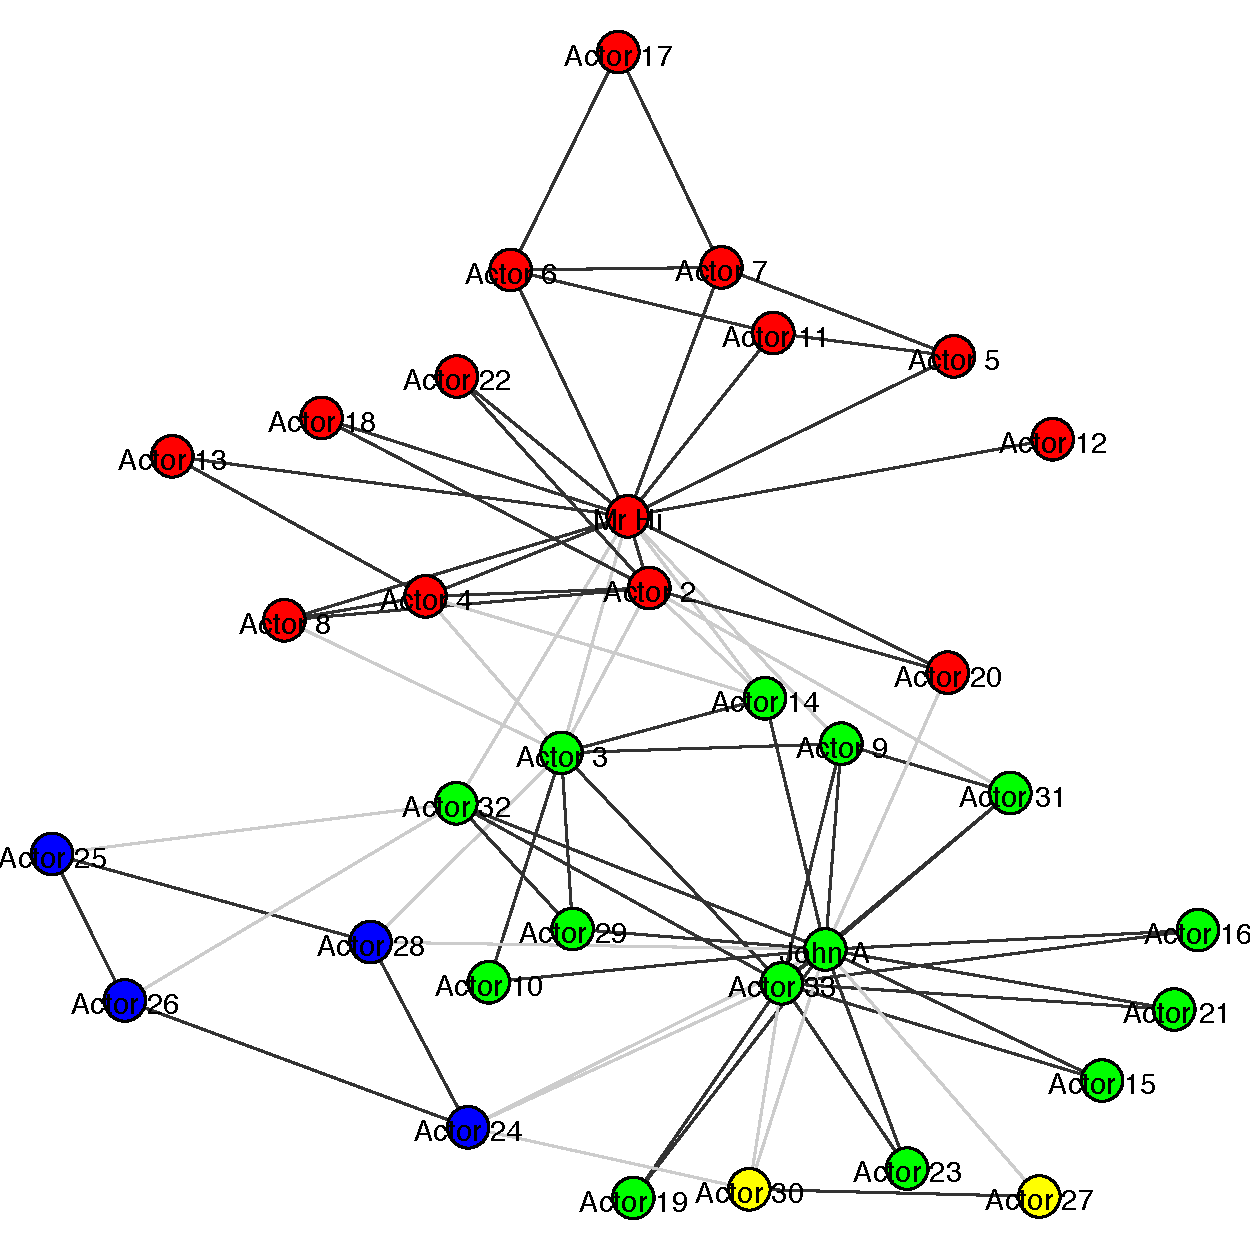
\includegraphics[scale=0.65]{q2/cluster4.pdf}}
\caption{4-Cluster Prediction}
\label{fig:cluster4}
\end{figure}

\begin{figure}[h!]
\centering
\fbox{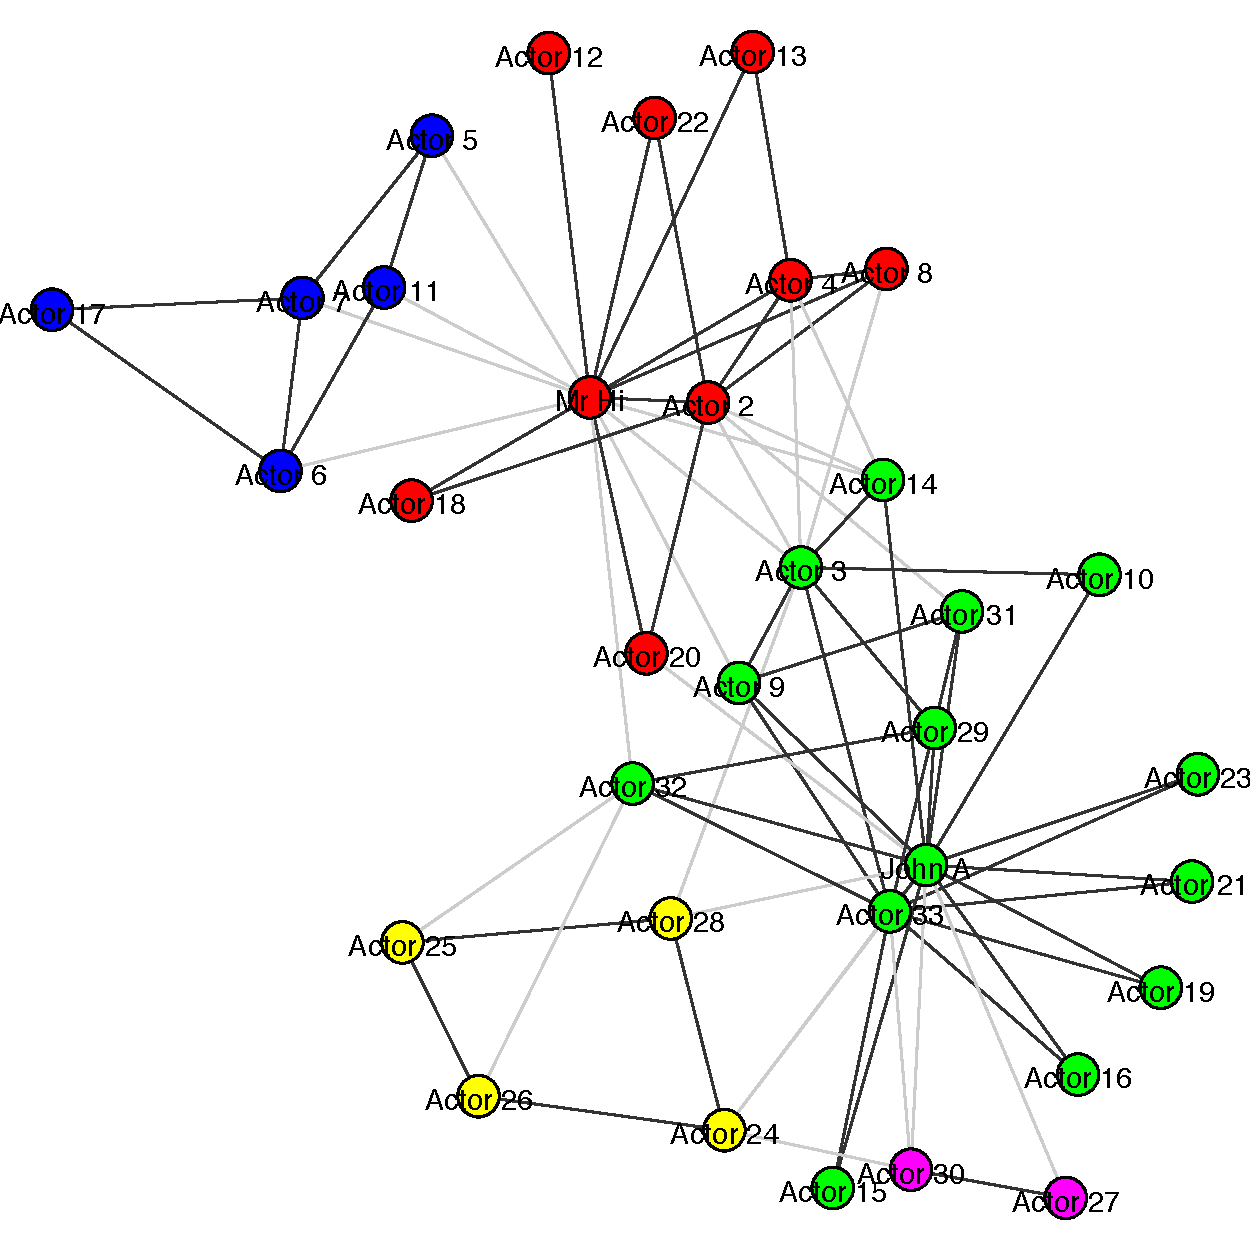
\includegraphics[scale=0.65]{q2/cluster5.pdf}}
\caption{5-Cluster Prediction}
\label{fig:cluster5}
\end{figure}
